\documentclass[a4paper, 11pt]{article}
\usepackage{comment} % enables the use of multi-line comments (\ifx \fi) 
\usepackage{lipsum} %This package just generates Lorem Ipsum filler text. 
\usepackage{fullpage} % changes the margin
\usepackage[utf8]{inputenc}
\usepackage{amsmath}
\usepackage{amsfonts}
\usepackage{graphicx}
\title{Mincost-flow-algoritmien suorituskykytestaus}
\author{Tuukka Korhonen}
\date{\today}
\begin{document}
\maketitle
\noindent

\section*{Algoritmit}
Testasin kolmea erilaista algoritmia mincost-maxflow ongelman ratkaisemiseen. 
\textsc{SAPSPFA} ja 
\textsc{SAPDijkstra} ovat lyhyimpiin augmentoiviin polkuihin perustuvia algoritmeja, jotka eivät toimi
yleisemmässä tapauksessa jossa verkossa voi olla negatiivisia syklejä. \textsc{ScalingCirculation} on
polynomisessa ajassa toimiva algoritmi joka toimii myös yleisemmässä tapauksessa.

\section*{Verkot}
Testasin mincost-flow algoritmien suorituskykyä viidellä erillaisella verkkotyypillä.
Neljä näistä verkkotyypeistä on satunnaisia verkkoja, jotka on generoitu eri tavoin. 
Yleisesti testejä voi luokitella neljän eri parametrin mukaan:
$n$, solmujen määrä, $m$, kaarien määrä, $U$, kaaren maksimikapasiteetti ja
$C$, kaaren maksimihinta. Lisäksi on verkkotyyppi joka on suunniteltu näyttämään 
ei-skaalaavien algoritmien pahin tapaus, jossa ne siis käyttäytyvät eksponentiaalisesti.
Generoin kaikissa satunnaistesteissä 50 erilaista testiä jokaista mittauspistettä kohti ja otin niiden suoritusaikojen
keskiarvon.

\section*{Teoreettinen aikavaativuus}
 \textsc{SAPSPFA} ja 
\textsc{SAPDijkstra} tarvitsevat pahimmassa tapauksessa $O(Um)$ augmentoivaa polkua joten niiden
aikavaativuudet ovat $O(Um^2 n)$ ja $O(Um^2 \log n)$. \textsc{ScalingCirculation} algoritmin
aikavaativuus on $O(m^2 \log n \log U)$, joka on polynominen aikavaativuus toisin kuin aiemmin mainitut.

\section*{Harvat verkot}
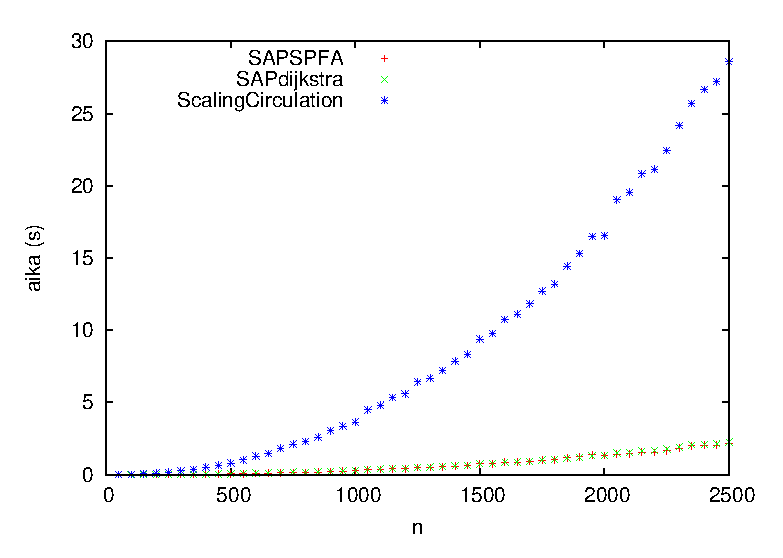
\includegraphics[scale=1.4]{application/random/sparse.eps}\\
Satunnaisgeneroituja verkkoja jotka generoitiin laittamalla $rand(2n, 3n)$ kaarta satunnaisten solmujen
välille, $n$ kaarta lähdesolmusta satunnaisiin solmuihin ja $n$ kaarta satunnaisista solmuista viemärisolmuun
 Kaarien kapasiteetit ovat satunnaislukuja väliltä $[1, 10000]$ ja hinnat satunnaislukuja
väliltä $[1, 1000]$. Näissä testeissä siis $m = O(n)$, $U = 10000$ ja $C = 1000$.

\section*{Tiheät verkot}
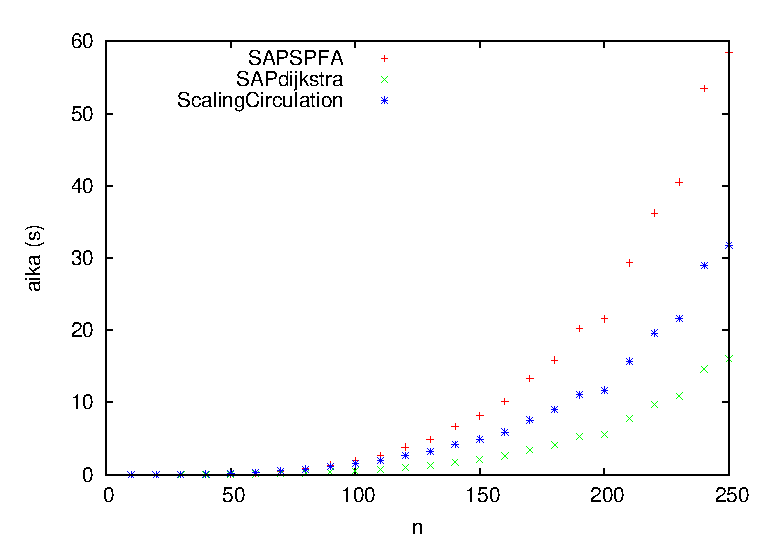
\includegraphics[scale=1.4]{application/random/dense.eps}\\
Satunnaisgeneroituja verkkoja jotka generoitiin laittamalla $rand(n^2, 2n^2)$ kaarta satunnaisten solmujen
välille, $n$ kaarta lähdesolmusta satunnaisiin solmuihin ja $n$ kaarta satunnaisista solmuista viemärisolmuun.
Kaarien kapasiteetit ovat satunnaislukuja väliltä $[1, 1000]$ ja hinnat satunnaislukuja väliltä
$[1, 1000]$. Näissä testeissä siis $m = O(n^2)$, $U = 1000$ ja $C = 1000$.

\section*{Harvat yksikkökapasiteettiverkot}
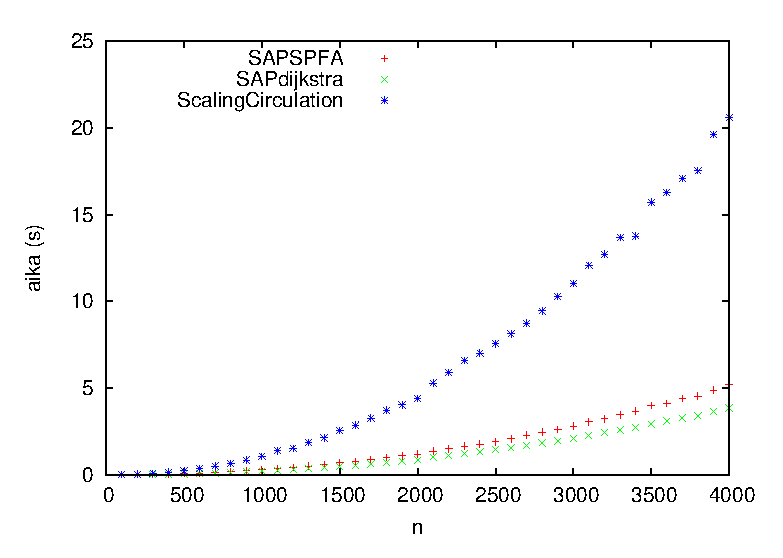
\includegraphics[scale=1.4]{application/random/sparseunitcap.eps}\\
Satunnaisgeneroituja verkkoja jotka generoitiin laittamalla $rand(4n, 6n)$ kaarta satunnaisten solmujen
välille, $n$ kaarta lähdesolmusta satunnaisiin solmuihin ja $n$ kaarta satunnaisista solmuista viemärisolmuun
 Kaarien kapasiteetit ovat $1$ ja hinnat satunnaislukuja
väliltä $[1, 1000]$. Näissä testeissä siis $m = O(n)$, $U = 1$ ja $C = 1000$.

\section*{Assignment problem}
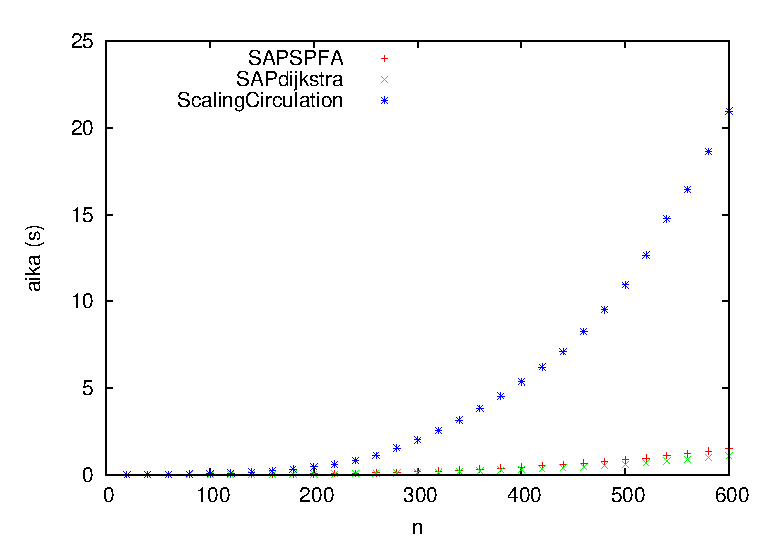
\includegraphics[scale=1.4]{application/random/assignment.eps}\\
Satunnaisgeneroituja \textsc{Assignment problem} ongelman instansseja mincost-maxflow muodossa. 
\textsc{Assignment problem} ongelmassa etsitään halvin täydellinen paritus täydellisessä 
kaksijakoisessa verkossa. Näissä
testeissä verkot olivat täydellisiä kaksijakoisia verkkoja joissa lähdesolmusta menee kaaret jokaiseen
toisen puolen solmuun ja jokaisesta toisen puolen solmusta kaaret viemärisolmuun. Kaikkien kaarien kapasiteetit
ovat $1$ ja hinnat satunnaislukuja väliltä $[1, 1000]$. Näissä testeissä siis $m = O(n^2)$, $U = 1$ ja $C = 1000$.

\section*{Vastaesimerkki}
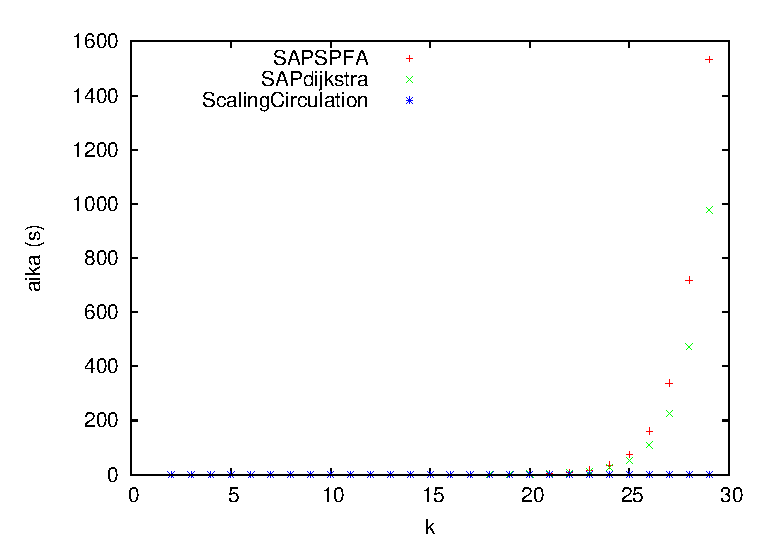
\includegraphics[scale=1.4]{application/random/pathological.eps}\\
Näissä verkoissa on erityinen konstruktio jolla \textsc{SAPSPFA} ja \textsc{SAPDijkstra} tarvii eksponentiaalisen
määrän augmentoivia polkuja. $n = 2k+2$, $m = 4k+1$, $U = 2^k$, $C = 2^k$.
\end{document}
